% !TEX root = main.tex

\chapter{Motivation}
\label{ch:motivation}
\noindent

\newcommand{\officialp}{official prose}
\newcommand{\spectecp}{SpecTec prose}


It might be easy to understand how the \officialp{} explains the control flow
of WebAssembly, if we assume that a WebAssembly code is loaded on a memory and
a pc points to the instruction to execute.
To describe control flow, it uses a structure named \textit{block} which
consitutes of a instruction sequence.
When executing the instructions in the block, pc can be changed to the starting
point of the block or the end of the block.

\textbf{Example 1}
\begin{verbatim}
  // infinite loop
  (loop (result i32) (i32.const 42) (br 0) (unreachable) end)
\end{verbatim}

Example 1 is a WebAssembly code example that has a \texttt{loop} whose result
type is \texttt{i32} and has a block of three instructions: \texttt{i32.const},
\texttt{br}, \texttt{unreachable}.
\cref{loop-fig} is the \officialp{} of the \texttt{loop} instruction.
It says that the continuation is the start of the loop, the information is
stored in a label, and it \textit{enters} the block with the label.
The term \textit{enter} means that it pushes the label in the stack and makes
pc points to the first instruction in the block.
The \texttt{i32.const} instruction is executed first, which just pushes the
\texttt{i32} value \texttt{42} in the stack.
Then, The \texttt{br} instruction is executed.
\cref{br-fig} is the \officialp{} of the \texttt{br} instruction.
It pops the label from the stack, and makes pc points to the continuation of
the label, which is the start of the loop instruction.
As a result, the code example above is a infinite loop pushing \texttt{42}
forever.

\begin{figure}[h!]
    \centerline{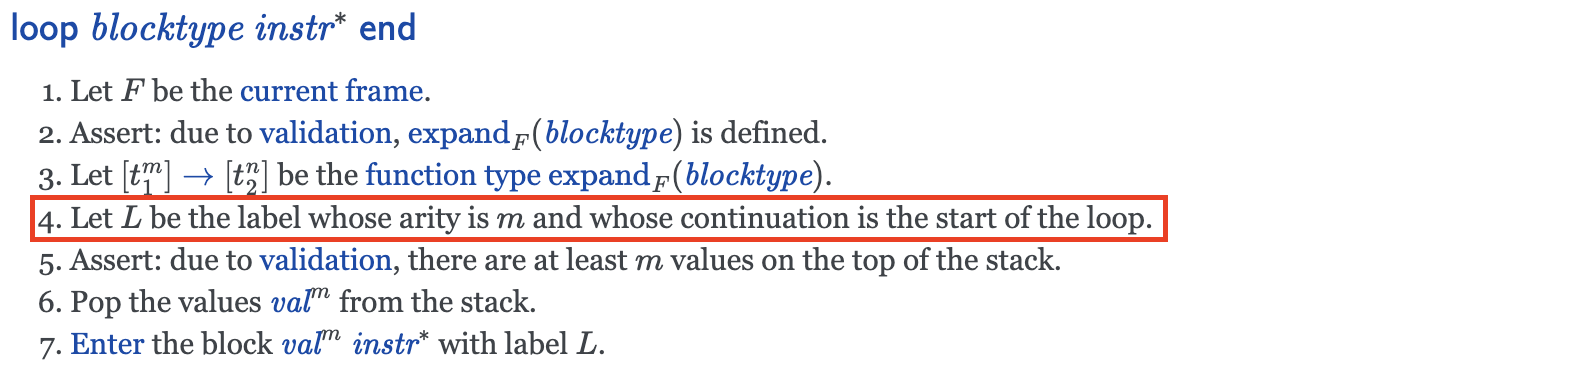
\includegraphics[width=15cm]{fig/loop}}
    \caption[Enter the caption title here]{\texttt{loop} instruction} \label{loop-fig}
    \centerline{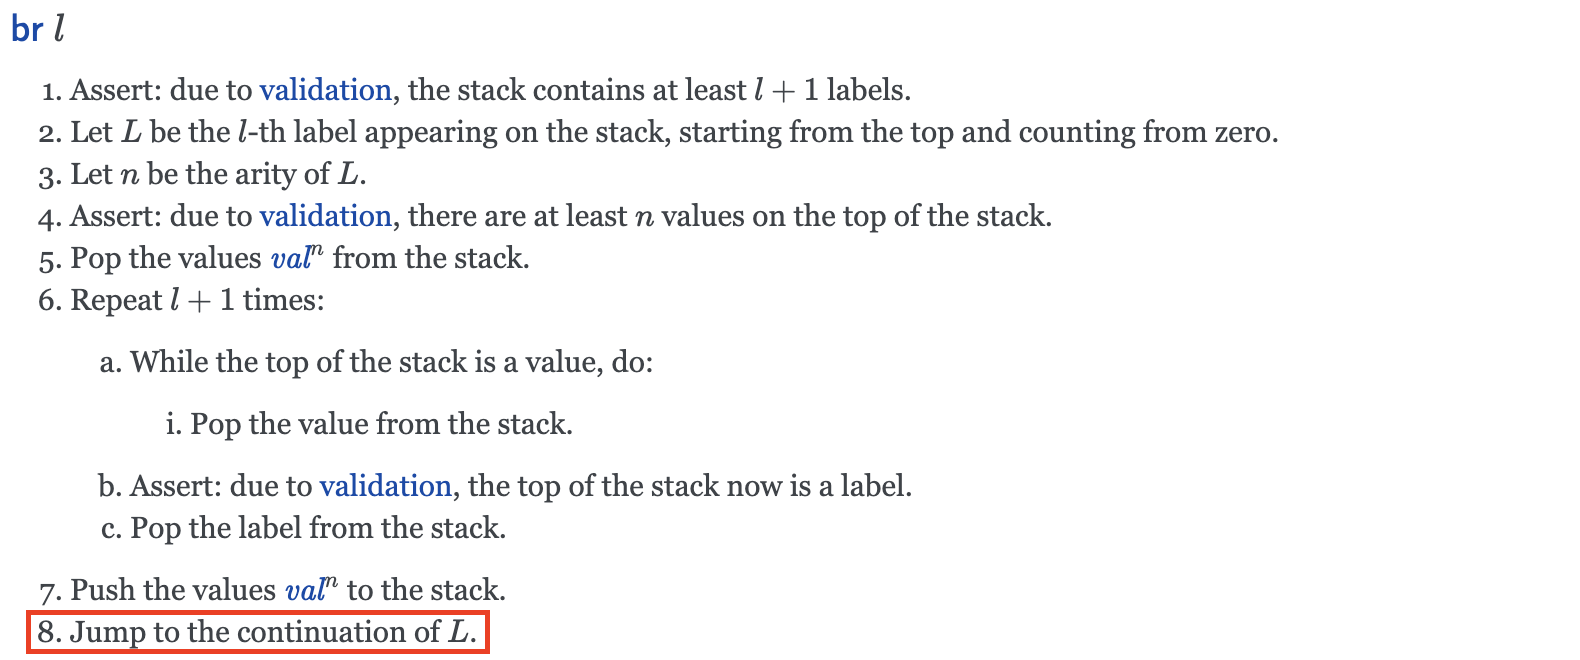
\includegraphics[width=15cm]{fig/br}}
    \caption[Enter the caption title here]{\texttt{br} instruction} \label{br-fig}
\end{figure}
TODO: remove redundant part in the fig

Similar to the control flow using the block and the label, there are many other
control instructions and structures such as a \texttt{call} instruction that
calls a function with a frame and a \texttt{return} instruction that returns from
the function with the frame.


TODO: detailed explanation of \spectecp{} w/ fig

However, the \spectecp{} assumes that the \red{machine} takes WebAssembly
instructions one by one, and changes the internal state accordingly without pc.
This is because the \spectecp{} is generated automatically from the \red{dsl}
which uses rewrite rule to describe WebAssembly semantics.
As a result, rather than jump to the start of the loop, \spectecp{} stores the
\texttt{loop} instruction itself in the label, and executes it again if the
\texttt{br} instruction is executed.
Not only that, it doesn't have block structure.

don't remember end!





% official spec prose notation control structure
% seems to be pc-based
% AL from DSL ~ formal notation: no pc
% AL: instruction sequence input continously
% device exit semantics for AL
% Executable spec passes all wasm testcases
% weird, maybe not happened in realworld, but valid wasm code
% wrong!
